%% Copyright (C) 2012 Minh Van Nguyen <mvngu.name@gmail.com>
%% This work is licensed under a the GNU Free Documentation License version
%% 1.3.  For the full terms of the license, see
%% http://www.gnu.org/licenses/fdl.html

\documentclass{beamer}

\usepackage{mystyle}


%%%%%%%%%%%%%%%%%%%%%%%%%%%%%%%%%%%%%%%%%%%%%%%%%%%%%%%%%%%%%%%%%%%%%%%%%%%

\title[Evolution of communities]{
  Community evolution in a scientific collaboration network
}
\institute{
  \large $^1$University of Melbourne, $^2$CSIRO
}
\author[Nguyen~et~al.]{
  Minh Van Nguyen,$^1$ Michael Kirley,$^1$ and \\
  Rodolfo Garc\'ia-Flores$^2$
}
%% uncomment the following line for the current date
\date{\small \today}
%% \date{}


%%%%%%%%%%%%%%%%%%%%%%%%%%%%%%%%%%%%%%%%%%%%%%%%%%%%%%%%%%%%%%%%%%%%%%%%%%%

\begin{document}

\frame{\titlepage}


%%%%%%%%%%%%%%%%%%%%%%%%%%%%%%%%%%%%%%%%%%%%%%%%%%%%%%%%%%%%%%%%%%%%%%%%%%%

%% Uncomment this section for the table of contents.
%% \frame{
%%   \frametitle{Contents}
%%   \tableofcontents
%% }


%%%%%%%%%%%%%%%%%%%%%%%%%%%%%%%%%%%%%%%%%%%%%%%%%%%%%%%%%%%%%%%%%%%%%%%%%%%

\section{Introduction}
%%
\frame{
  \frametitle{Introduction}
  %%
  \begin{itemize}
  \item The presence of communities in social networks is intuitive.
    %% Think of members of a social club such as a sports club, a
    %% professional association such as the ACM, the developers of a
    %% software project, or online communities such as Facebook
    %% groups.  The concept of communities can also be transferred to
    %% other types of networks.  In a financial or economic network, a
    %% community might be a group of organizations that trade more
    %% amongst themselves than with other organizations.  In a
    %% software network, a community might be a group of functions or
    %% modules that invoke each other more often than other functions
    %% or modules in a software package.
  \end{itemize}

  \begin{figure}[!bp]
  \centering
  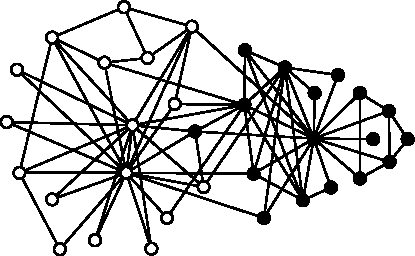
\includegraphics{image/Zachary-karate-club-community}
  \caption{Two communities in a karate club~\cite{Zachary1977}.}
  \end{figure}
}


%%%%%%%%%%%%%%%%%%%%%%%%%%%%%%%%%%%%%%%%%%%%%%%%%%%%%%%%%%%%%%%%%%%%%%%%%%%

\section{Motivation and aim}
%%
\frame{
  \frametitle{Motivation and aim}
  %%
  \begin{itemize}
  \item Uncover principles of community evolution.
    \begin{itemize}
    \item Understand how a blog network evolve~\cite{LinEtAl2008}
    \item Discover calling patterns \& customer churns in a mobile
      phone network~\cite{GreeneEtAl2010,PallaEtAl2007}
    \item Map out the long-term collaboration among groups of
      researchers~\cite{PallaEtAl2007}
    \end{itemize}

  \item How does community size affect the evolution of communities?
    %% The above general question can be answered along two separate
    %% lines.  One is to focus on the scaling characteristic of
    %% community size and any implication that this has for the
    %% long-term statistical properties of communities.  Another is to
    %% focus on any effects that the minimum community size has on
    %% events in the history of communities.
    \begin{itemize}
    \item What is the scaling characteristic of community size and the
      implication for community evolution?
      %% This relates to the long-term behaviour of the distribution
      %% of community size.

    \item How does the minimum size of communities affect the
      life-cycle of communities?
      %% This is about exploring the relationship between minimum
      %% community size and events in the history of communities.

    %% \item To what extent can the minimum community size be used to
    %%   filter out inactive communities?
    \end{itemize}
  \end{itemize}
}


%%%%%%%%%%%%%%%%%%%%%%%%%%%%%%%%%%%%%%%%%%%%%%%%%%%%%%%%%%%%%%%%%%%%%%%%%%%

\section{Background}

\frame{
  \frametitle{Background}
  %%
  \begin{itemize}
  \item Communities evolve according to a
    life-cycle~\cite{GreeneEtAl2010,PallaEtAl2007}:
    \begin{itemize}
    \item birth \& death

    \item expand \& contract

    \item merge \& split
    \end{itemize}

  \item Communities are matched across time in order to infer the
    history of a ``dynamic community'' from birth to death.
  \end{itemize}

  \begin{figure}
  \centering
  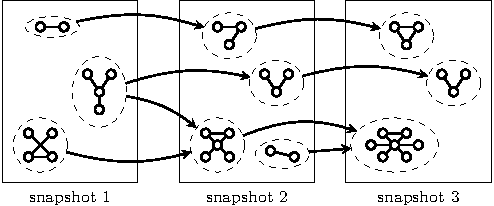
\includegraphics{image/match}
  \caption{The evolution of communities in terms of a life-cycle model.}
  \end{figure}
}


%%%%%%%%%%%%%%%%%%%%%%%%%%%%%%%%%%%%%%%%%%%%%%%%%%%%%%%%%%%%%%%%%%%%%%%%%%%

\section{Our contributions}

\frame{
  \frametitle{Our contributions}
  %%
  \begin{itemize}
  \item The parameter $s_{\min}$, the minimum community size.

  \item An extended-life cycle model.
    \begin{itemize}
    \item direct: two communities match only each other

    \item missing: a community is dormant at a particular snapshot

    \item resume: a dormant community appears again

    \item stable: relatively little change in size between two
      consecutive snapshots

    \item stagnant: no change in size at all between two consecutive
      snapshots
    \end{itemize}
  \end{itemize}
}


%%%%%%%%%%%%%%%%%%%%%%%%%%%%%%%%%%%%%%%%%%%%%%%%%%%%%%%%%%%%%%%%%%%%%%%%%%%

\section{Experiments and methods}

\frame{
  \frametitle{Experiments and methods}
  %%
  \begin{itemize}
  \item We constructed from the Genetic Programming~(GP) bibliography
    yearly snapshots of a network of scientific co-authorship.

  \item From each snapshot, we extracted communities using the
    algorithm of Blondel~et~al.~\cite{BlondelEtAl2008a}.  We also used
    the algorithm of Raghavan~et~al.~\cite{RaghavanEtAl2007}.

  \item Communities were matched using the Jaccard coefficient
    $J(A,B) = |A \cap B| \big/ |A \cup B|$ to compute a measure of
    overlap.

  \item Two communities match each other if they had an overlap score
    of $J(A,B) > 0.3$.  In that case, we treated $A$ and $B$ as nodes
    and created a directed edge from $A$ to $B$.

  \item Extract the history of each dynamic community by doing
    depth-first searches from communities that occurred in the
    earliest snapshots, and work our way up to communities that
    occurred in the latest snapshots.
  \end{itemize}
}


%%%%%%%%%%%%%%%%%%%%%%%%%%%%%%%%%%%%%%%%%%%%%%%%%%%%%%%%%%%%%%%%%%%%%%%%%%%

\section{Results}

\frame{
  \frametitle{Results: distribution of community size}
  %%
  \begin{itemize}
  \item The distribution of community size follows a power-law of the
    form $p_k \sim k^{-\alpha}$.  This suggests the presence of
    self-similarity in the GP co-authorship network.
    %% Self-similarity is a typical feature of fractals.  In the long
    %% run, a power-law regime suggests that the larger is a community
    %% of GP co-authors, the more likely that the community would
    %% attract new co-authors.
  \end{itemize}

  \begin{figure}
  \centering
  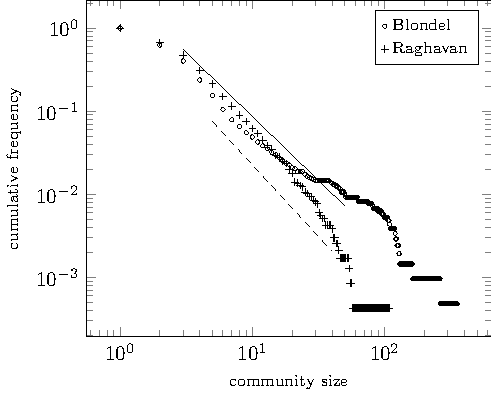
\includegraphics[scale=0.8]{image/noeditors-commsize-dist}
  \caption{Power-law regime in the distribution of community size,
    where $\alpha \approx 2.54$~(solid line) and
    $\alpha \approx 2.72$~(dashed line).}
  \end{figure}
}


%%%%%%%%%%%%%%%%%%%%%%%%%%%%%%%%%%%%%%%%%%%%%%%%%%%%%%%%%%%%%%%%%%%%%%%%%%%

\bibliographystyle{bibliography.bst}
\bibliography{bibliography}

\end{document}
